%%%%%%%%%%%%%%%%%%%%%%%%%%%%%%%%%%%%%%%%%%%%%%%%%%%%%%%%%%%%
%%% ELIFE ARTICLE TEMPLATE
%%%%%%%%%%%%%%%%%%%%%%%%%%%%%%%%%%%%%%%%%%%%%%%%%%%%%%%%%%%%
%%% PREAMBLE 
\documentclass[9pt,lineno]{elife}
% Use the onehalfspacing option for 1.5 line spacing
% Use the doublespacing option for 2.0 line spacing
% Please note that these options may affect formatting.

\usepackage{lipsum} % Required to insert dummy text
\usepackage[version=4]{mhchem}
\usepackage{siunitx}
\DeclareSIUnit\Molar{M}

%%%%%%%%%%%%%%%%%%%%%%%%%%%%%%%%%%%%%%%%%%%%%%%%%%%%%%%%%%%%
%%% ARTICLE SETUP
%%%%%%%%%%%%%%%%%%%%%%%%%%%%%%%%%%%%%%%%%%%%%%%%%%%%%%%%%%%%
\title{Transcriptional dynamics of influenza virus infection at the single-cell level}

\author[1]{Alistair B. Russell}
\author[2]{Cole Trapnell}
\author[1,2*]{Jesse D. Bloom}
\affil[1]{Basic Sciences Division and Computational Biology Program, Fred Hutchinson Cancer Research Center, Seattle, United States}
\affil[2]{Department of Genome Sciences, University of Washington, Seattle, United States}
\corr{jbloom@fredhutch.org}{}

% \presentadd[\authfn{5}]{eLife Sciences editorial Office, eLife Sciences, Cambridge, United Kingdom}

%%%%%%%%%%%%%%%%%%%%%%%%%%%%%%%%%%%%%%%%%%%%%%%%%%%%%%%%%%%%
%%% ARTICLE START
%%%%%%%%%%%%%%%%%%%%%%%%%%%%%%%%%%%%%%%%%%%%%%%%%%%%%%%%%%%%

\begin{document}

\maketitle

\begin{abstract}
Influenza virus infection induces large changes in cellular transcription.
Previously this has mostly been looked at using bulk measurements
Here we examine the process at the level of single cells.
We find extremely wide variation in the extent of viral gene transcription across infected cells.
IFN induction is very rare.
Some cellular pathways may be consistently altered in cells with high burden of viral transcripts.
Overall, highlights remarkable heterogeneity in the outcome of infection.
\end{abstract}

\section{Key background references}
Here we list some key background references on some relevant points.

\subsection{Stochasticity during viral infection}

\subsection{Influenza co-infection and defective particles}

\subsection{Interferon induction}

\subsection{Transcriptional dynamics}

\subsection{Single-cell studies}

\section{Introduction}

Your introduction goes here!
\emph{Put each sentence on a separate line to enable tracking with git.}

Here's a second paragraph to test paragraph indents. \lipsum[1]

\section{Results}

\subsection{Level 2 Heading}

\lipsum[3]

\begin{figure}
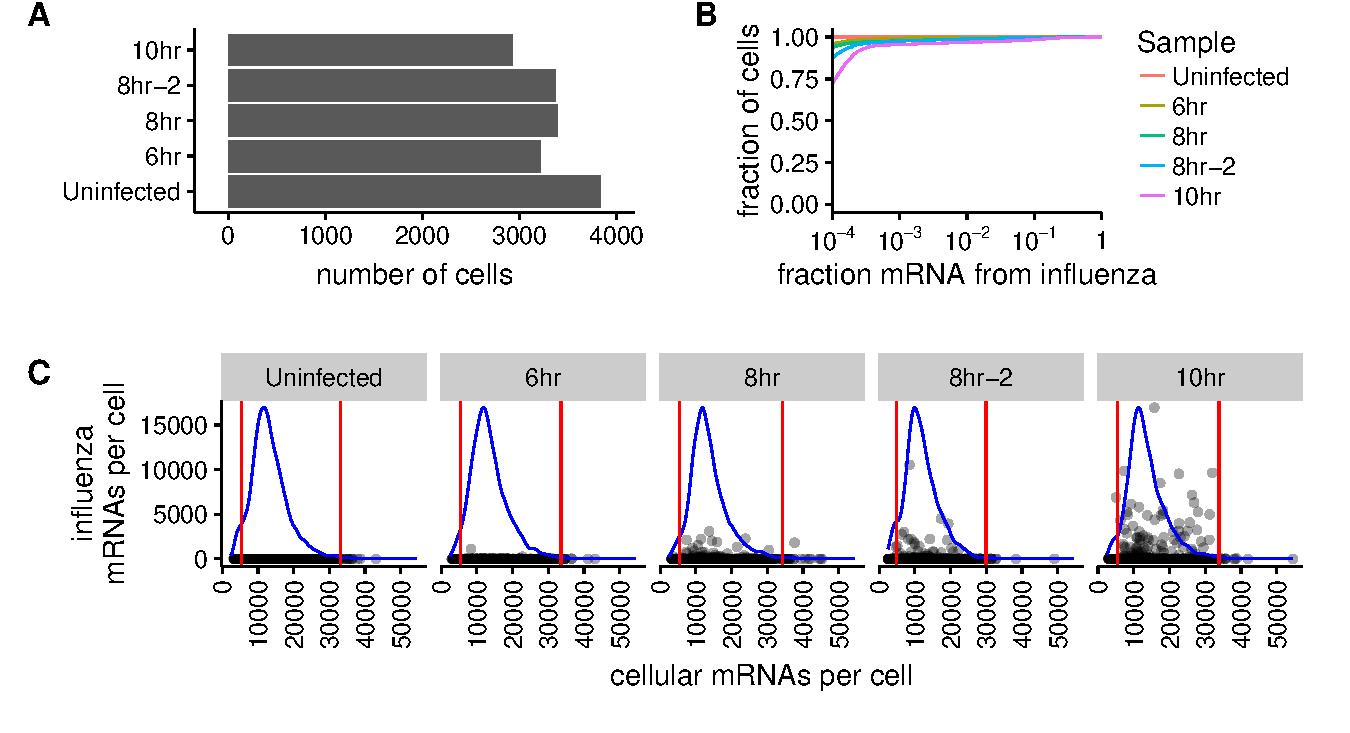
\includegraphics[width=\linewidth]{figures/p_cell_mRNA_summary.pdf}
\caption{
Overview of amounts of cellular and influenza virus mRNAs detected in each cell.
{\bf (A)} 
Number of cells captured for each sample.
{\bf (B)} 
Cumulative fraction plot showing the amount of mRNA derived from influenza for each sample.
In all samples, most cells had little or no influenza mRNA.
{\bf (C)} 
The number of cellular and viral mRNAs for each cell is plotted as a point.
The blue lines show the overall distribution of the number of cellular mRNAs per sample.
Cells that fell outside the red lines were removed as outliers.
At later timepoints, a small number of cells had a very high number of viral mRNAs.
}
\label{fig:cells}
\figsupp[Shorter caption for main text.]{This is a supplementary figure's full caption, which will be used at the end of the manuscript.}{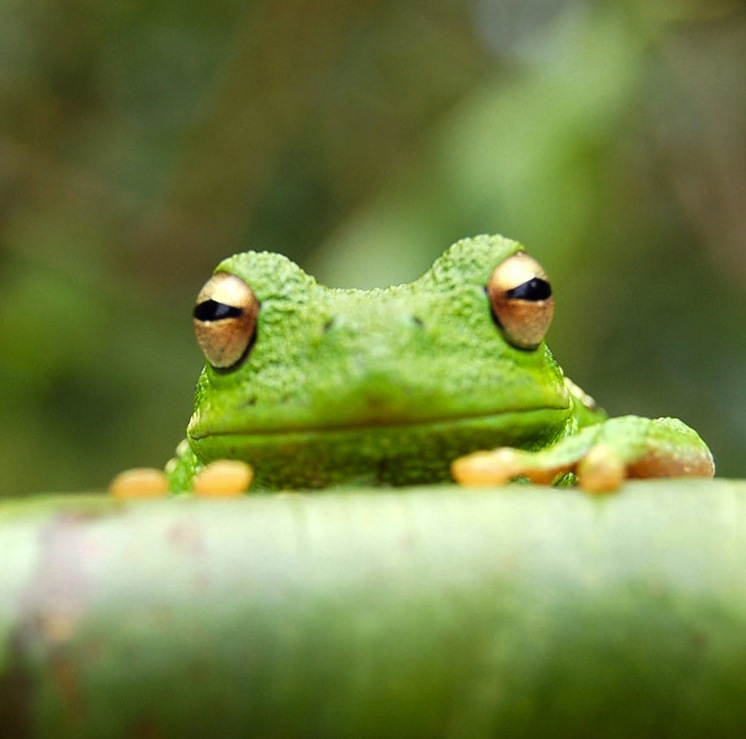
\includegraphics[width=6cm]{frog}}
\figsupp{This is another supplementary figure.}{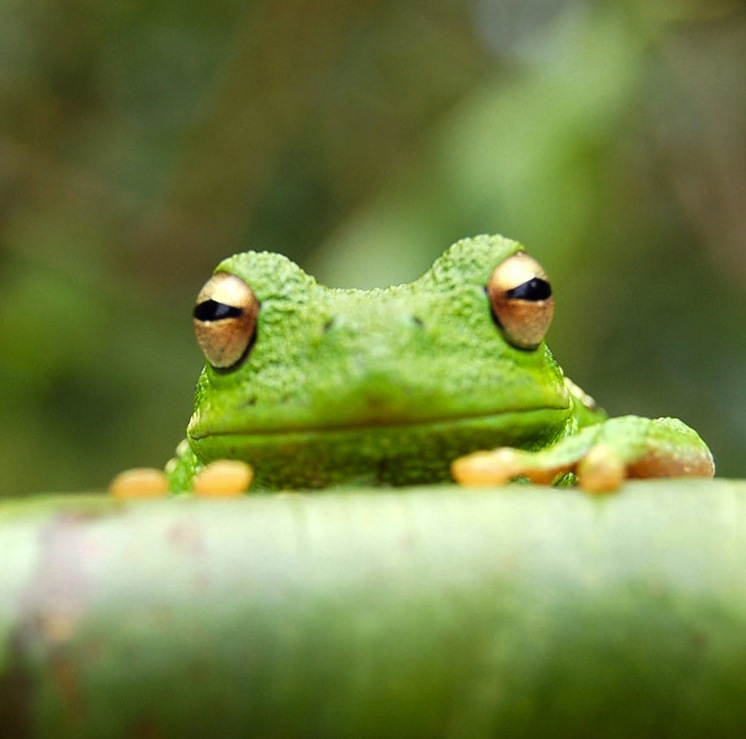
\includegraphics[width=6cm]{frog}}
\figdata{This is a description of a data source.}
\end{figure}

\begin{figure}
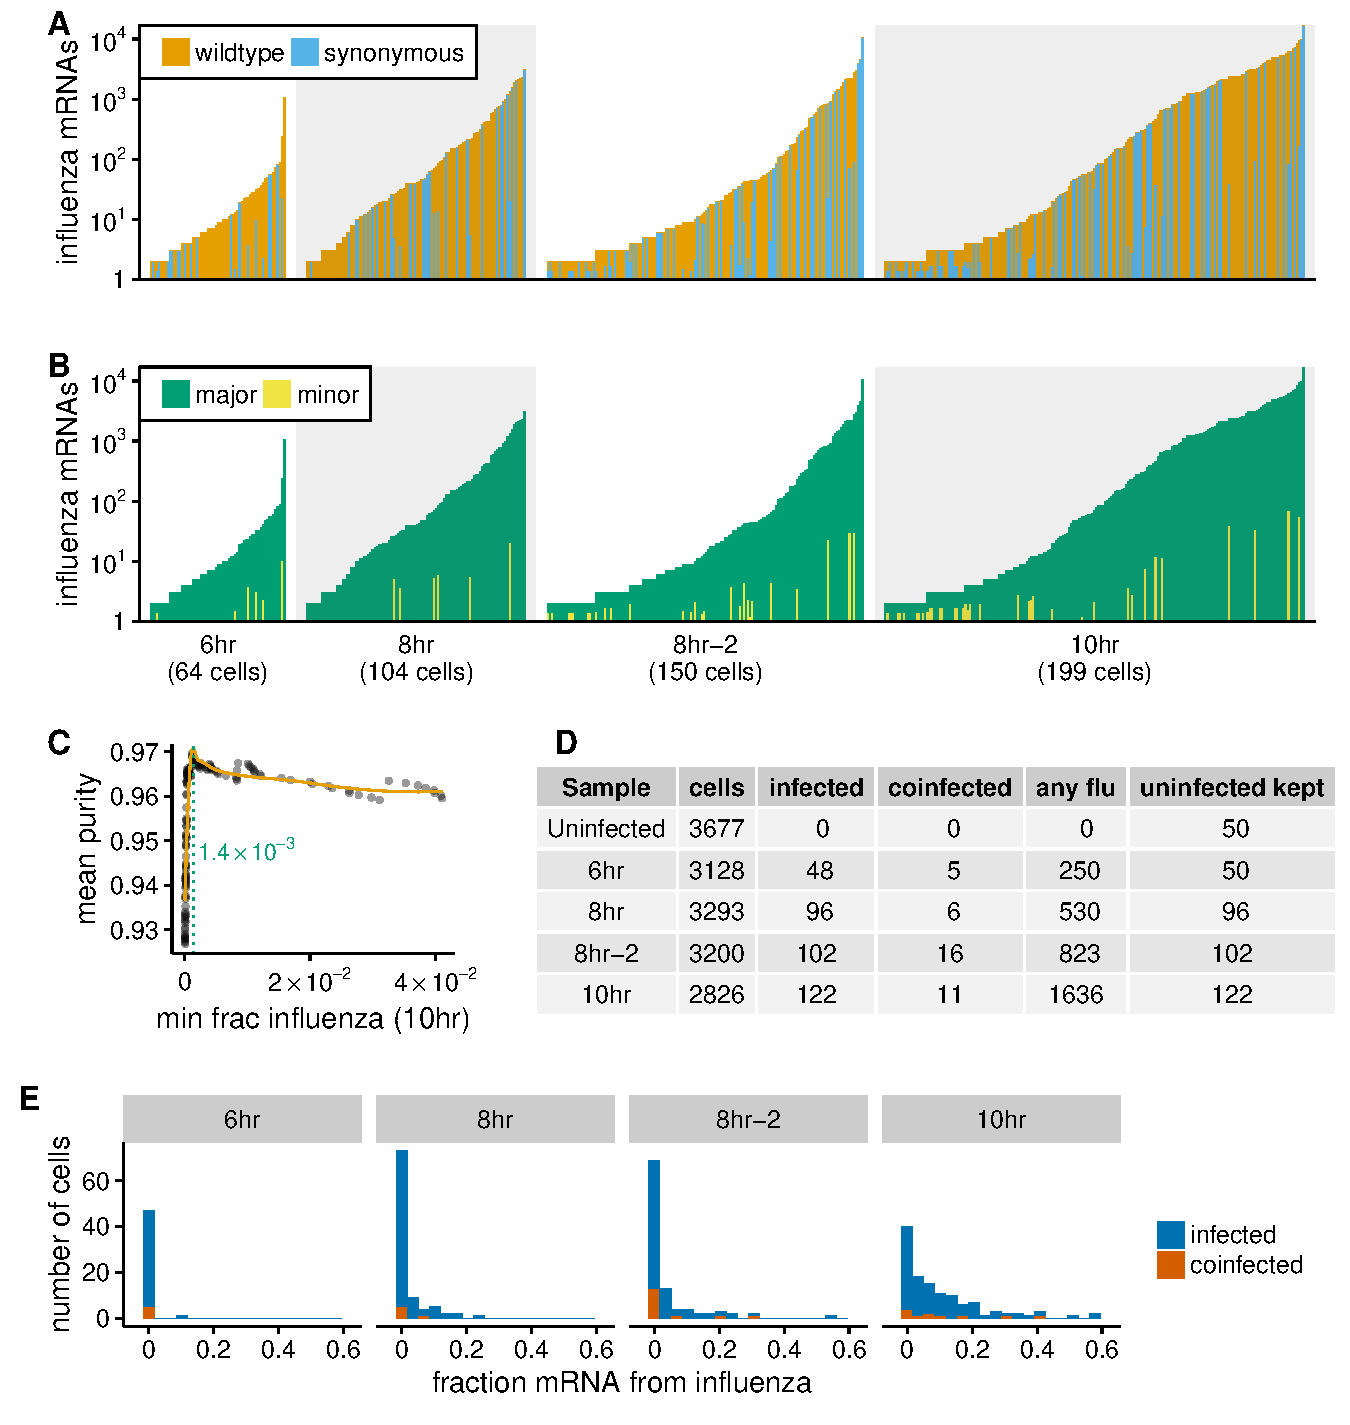
\includegraphics[width=\linewidth]{figures/p_frac_flu_summary.pdf}
\caption{
Synonymous barcodes near the 3' end of the influenza virus mRNAs were used to identify co-infection and distinguish true infections from cells that contained a few spurious viral reads.
{\bf (A)}
For all cells with at least two viral mRNAs for which the synonymous barcode could be called, each line is proportional to the logarithm of the number of viral mRNAs in that cell.
The bars are colored in linear proportion to the fraction of the viral mRNAs derived from either wildtype or synonymously barcoded virus.
{\bf (B)}
Same as (A), but now each bar is colored according to the relative proportions of the more common (major) and less common (minor) barcoded virus variant.
At low levels of viral mRNA there is often a roughly equal mix of barcodes, since many of these cells have simply picked up environment mRNA which is about equally likely to derive from either virus.
But at higher levels of viral mRNA, truly infected cells are mostly one pure barcode except for a few cells that are truly co-infected.
{\bf (C)}
We determined a cutoff for calling ``true'' infections by fitting a curve to the mean barcode purity of all cells with greater than a given fraction of their mRNA derived from virus.
We called the cutoff at the point at which purity stops increasing with the fraction of viral mRNA.
{\bf (D)}
The number of cells identified as infected and co-infected for each sample.
For all samples, the vast majority of cells were not infected, so for subsequent analyses we subsampled to a number of uninfected cells that was the greater of 50 or the number of infected cells.
{\bf (E)} 
The distribution of the fraction of mRNA derived from virus for each sample for both infected and co-infected cells.
For all samples, there is a very wide distribution of the amount of viral mRNA.
}
\label{fig:fracflu}
\end{figure}

\begin{figure}
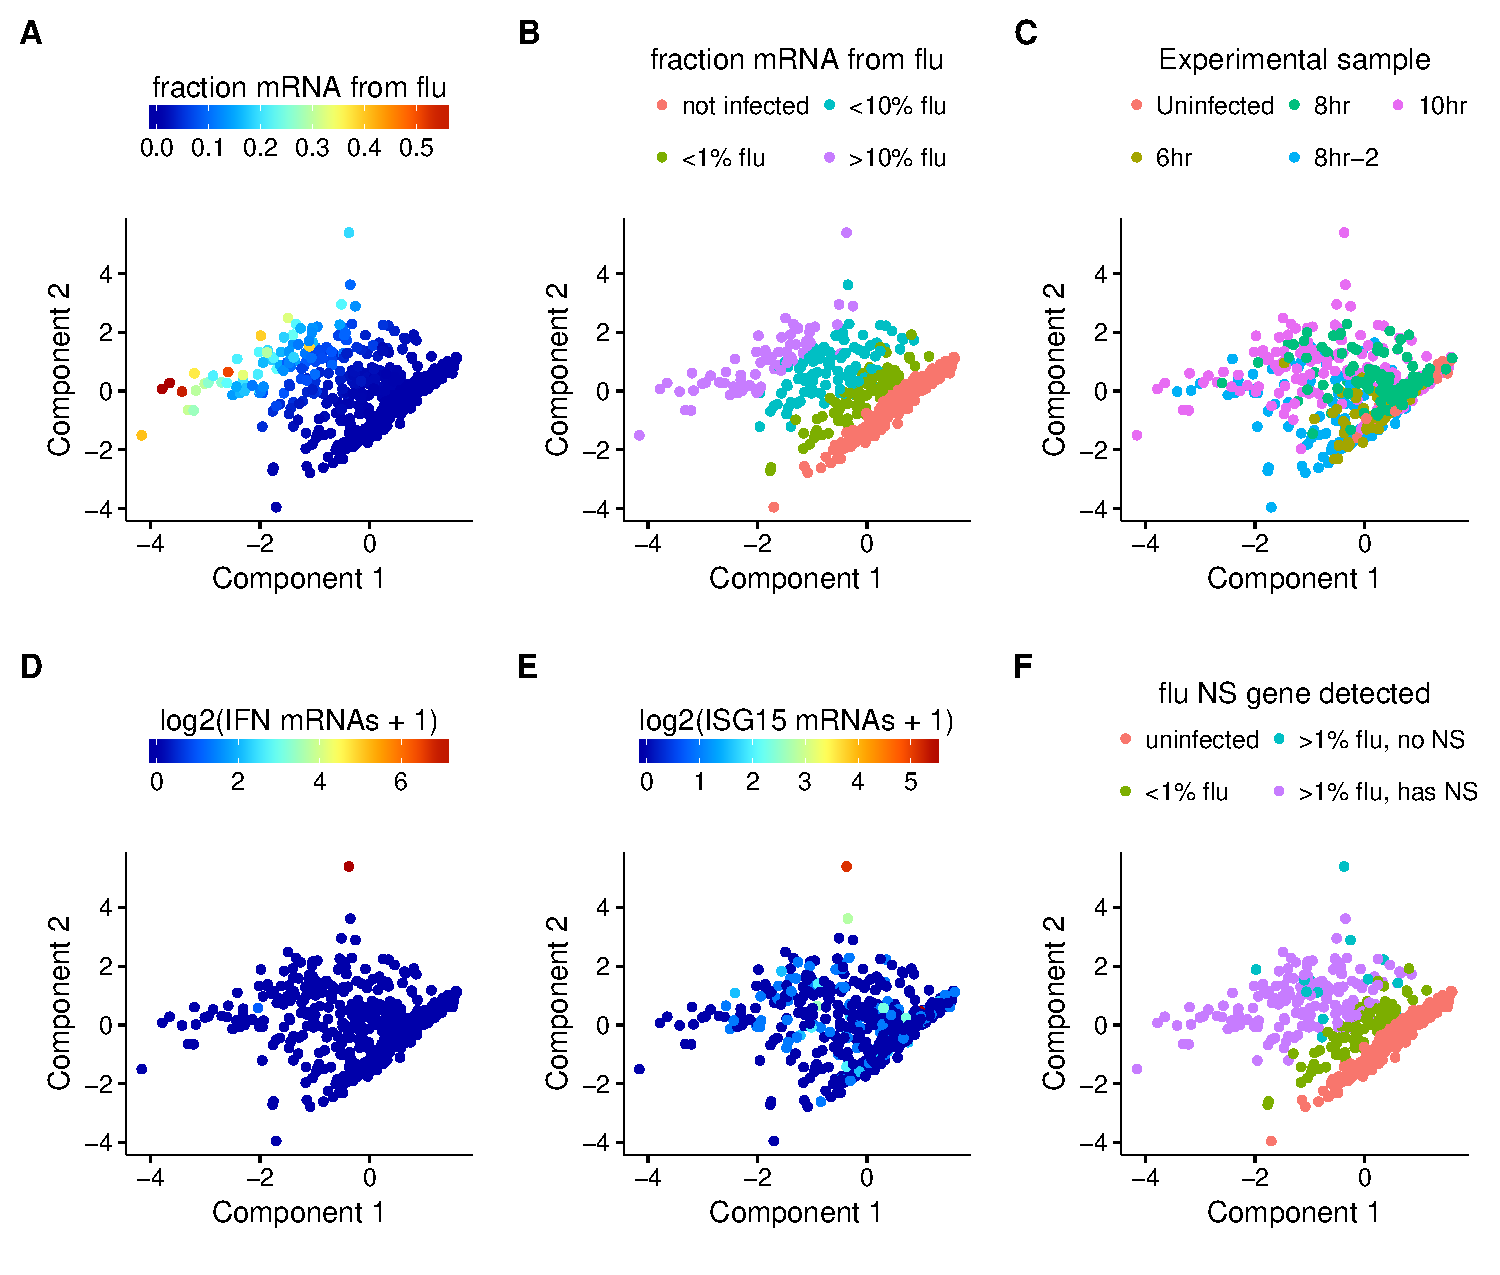
\includegraphics[width=\linewidth]{figures/p_pseudo_merge.pdf}
\caption{
Visual layout of the cells according to ``pseudotime''.
The layout is the same in all panels, but each panel colors the cells according to a different property.
{\bf (A), (B)}
Cells colored by the fraction of their mRNA that is viral.
{\bf (C)}
Cells colored by experimental sample.
While it is clear that cells from later timepoints often have more viral RNA, there are cells from earlier timepoints with a high viral burden and cells from late timepoints with a low viral burden.
{\bf (D)}
Cells colored by the number of type I and III interferon transcripts detected.
Only one cell has high expression of these interferons.
{\bf (E)}
Cells colored by the expression of the interferon-stimulate gene ISG15.
{\bf (F)}
For cells with at least 1\% of their reads from influenza, are the cells expressing the viral NS protein?
The one interferon-positive cell is lacking NS, but many other cells also lack NS but do not express interferon.
}
\label{fig:pseudotime}
\end{figure}

\begin{figure}
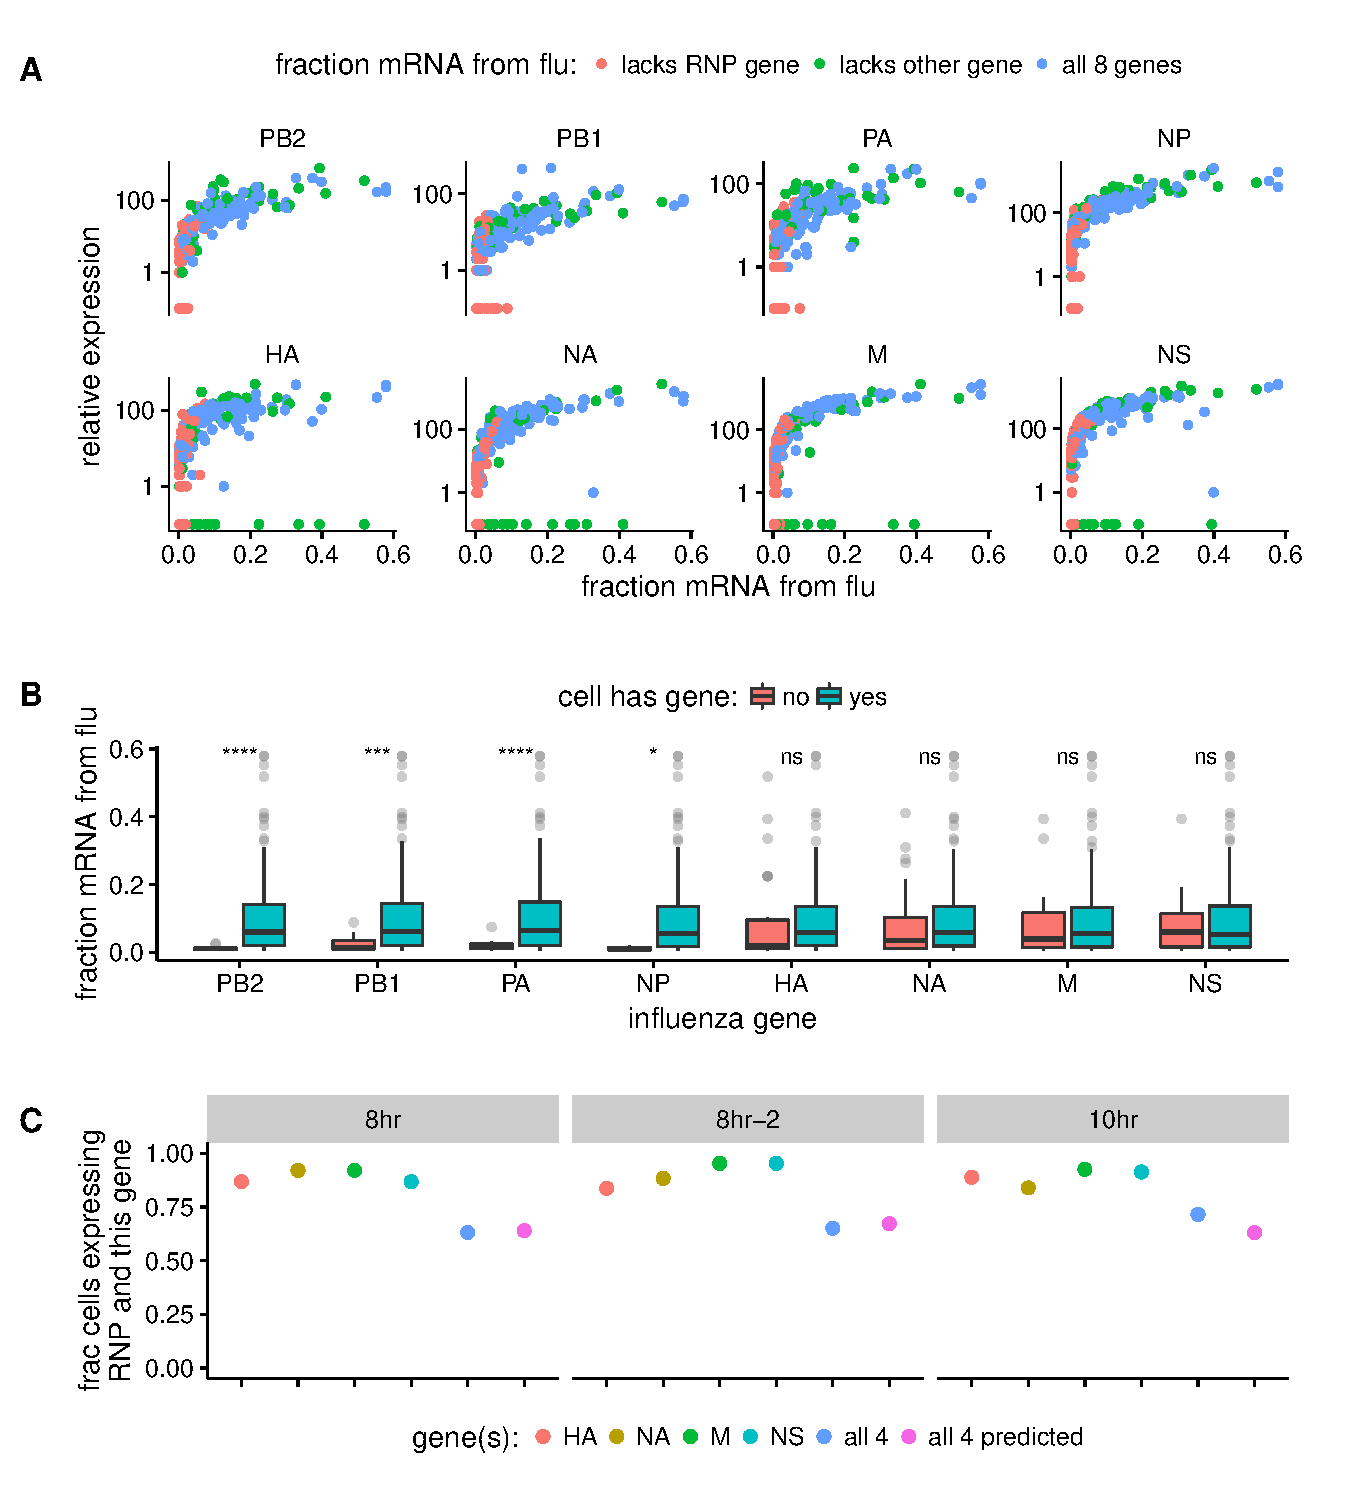
\includegraphics[width=\linewidth]{figures/p_flu_burden_flu_gene_merge.pdf}
\caption{
The viral infection burden in individual cells as a function of the amount of each viral gene detected.
{\bf (A)} 
Fraction of mRNAs in each cell derived from virus as a function of the \emph{normalized} expression of each viral gene in that cell.
This plot shows that all cells with very high viral burden express all of the RNP genes, but some cells with high viral burden lack each of the other four viral genes.
{\bf (B)}
Statistical tests confirming that absence of viral RNP genes is significantly associated with reduced viral burden, but that the absence of the non-RNP genes does not lead to a clear decrease in viral burden.
}
\label{fig:fluburdenbyflugene}
\end{figure}

\begin{figure}
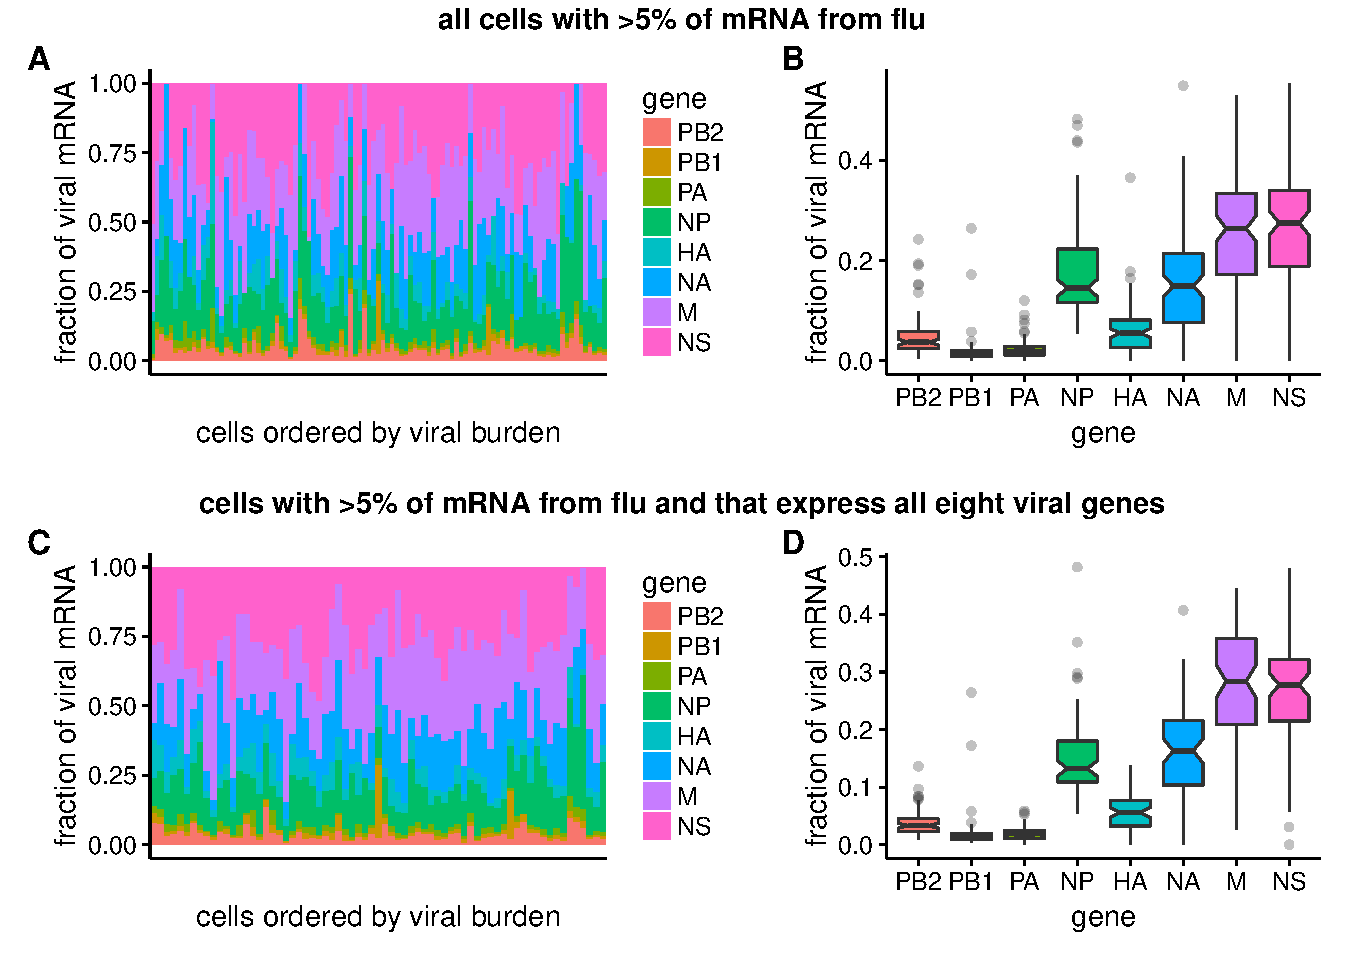
\includegraphics[width=\linewidth]{figures/p_flu_expr.pdf}
\caption{
Expression of individual influenza genes in highly infected cells (at least 5\% of total mRNA is viral).
{\bf (A)} 
The fraction of total mRNA from each influenza gene for each cell.
{\bf (B)}
Box plots showing the fraction of viral mRNA per cell that is derived from each influenza gene taken over all highly expressed cells.
The black line at the notch in each box is the median, and the top and bottom of the box indicate the first and third quartiles.
}
\label{fig:fluexpr}
\figdata{The raw data are in \texttt{p\_flu\_expr.csv}.}
\end{figure}

\begin{figure}
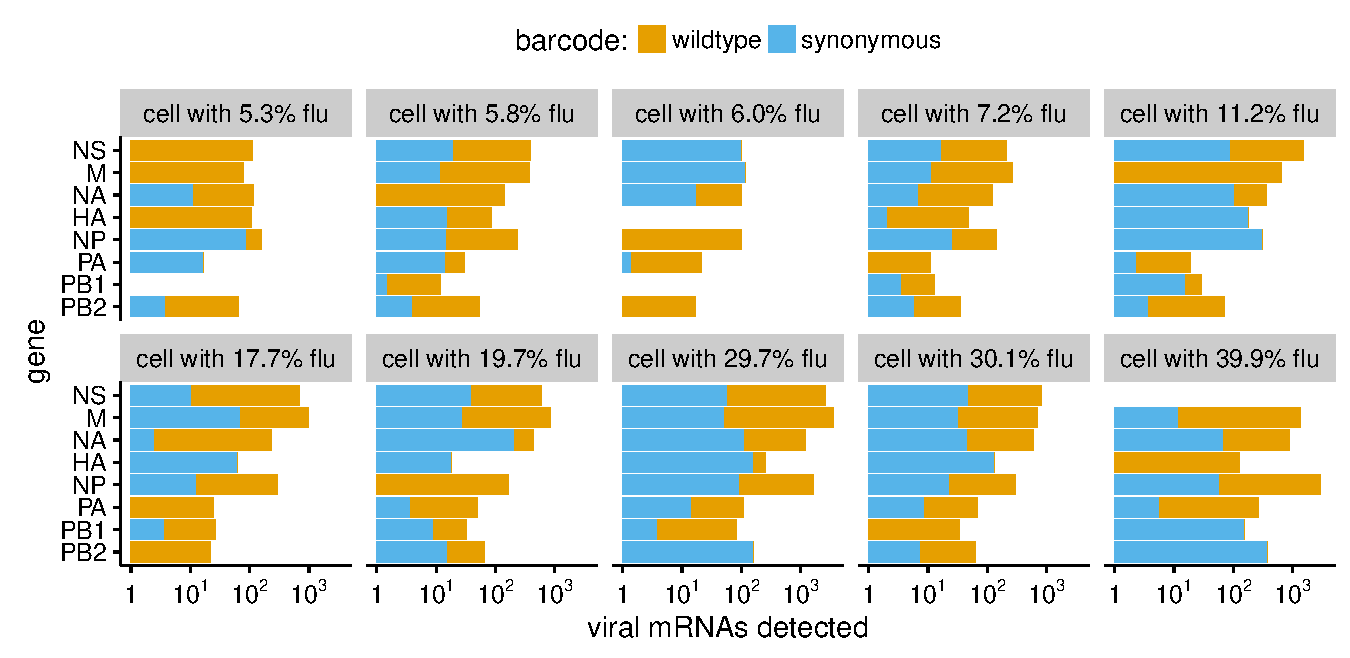
\includegraphics[width=\linewidth]{figures/p_coinfection.pdf}
\caption{
Frequency of each viral gene segment in co-infected cells with at least 5\% of their mRNA derived from influenza.
The bars indicate the logarithm of the number of each viral mRNA detected, and the bars are colored in proportion to the fraction of those mRNAs that are derived from either wildtype or synonymous barcoded virus.
}
\label{fig:coexpression}
\figdata{The raw data plotted in this figure are in \texttt{p\_coinfection.csv}.}
\end{figure}

\begin{figure}
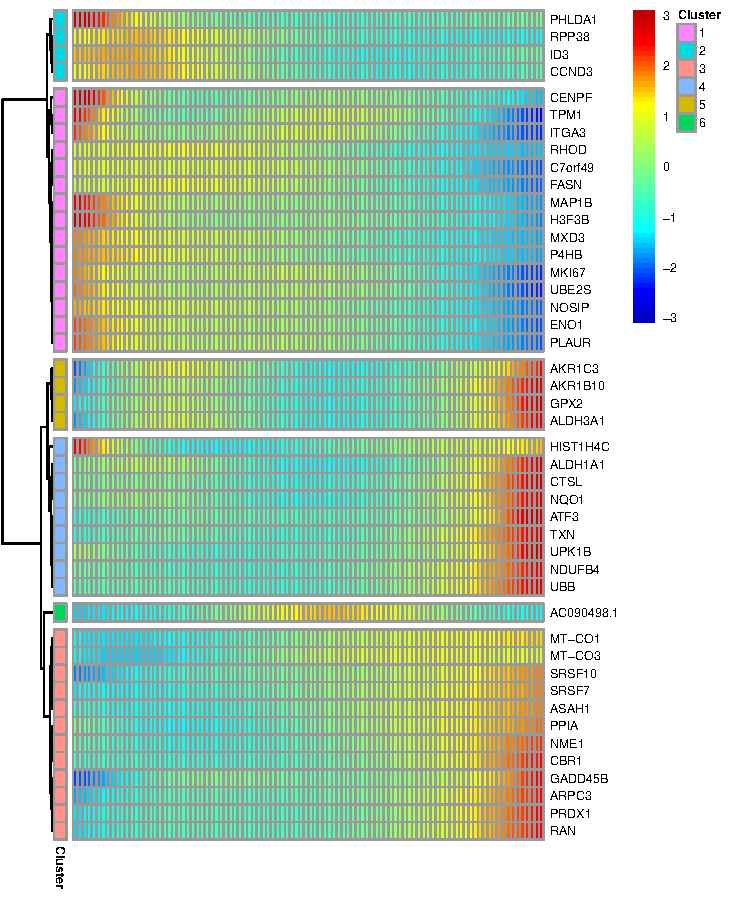
\includegraphics[width=0.8\linewidth]{figures/p_cellular_heatmap.pdf}
\caption{
Cellular genes that are differentially expressed with respect to the amount of influenza mRNA in individual cells infected with full influenza virus containing all eight genes.
Shown are all genes differentially expressed with $Q < 0.1$.}
\label{fig:cellulargenes}
\figdata{The full results of the differential expression test is in \texttt{p\_sig\_cellular\_genes.csv}.}
\figdata{The results of a gene-set analysis are in \texttt{p\_sig\_cellular\_genes.csv}.}
\end{figure}

\section{Discussion}

\lipsum[9]

\section{Methods and Materials}

Guidelines can be included for standard research article sections, such as this one. 

\lipsum[3]

\section{Some \LaTeX{} Examples}
\label{sec:examples}

Use section and subsection commands to organize your document. 
\LaTeX{} handles all the formatting and numbering automatically. 
Use ref and label commands for cross-references.

\subsection{Figures and Tables}


If you use the following prefixes for your \verb|\label|:
%
\begin{description}
\item[Figures] \texttt{fig:}, e.g.~\verb|\label{fig:view}|
\item[Tables] \texttt{tab:}, e.g.~\verb|\label{tab:example}|
\item[Equations] \texttt{eq:}, e.g.~\verb|\label{eq:CLT}|
\item[Boxes] \texttt{box:}, e.g.~\verb|\label{box:simple}|
\end{description}
%
you can then use the convenience commands as in \verb|\FIG{cells}|, \ to generate cross-reference \FIG{view}. 

\subsection{Citations}

LaTeX formats citations and references automatically using the bibliography records in your .bib file, which you can edit via the project menu. 
Use the \verb|\cite| command for an inline citation, like \cite{trapnell2014pseudo}, and the \verb|\citep| command for a citation in parentheses \citep{trapnell2014pseudo}. 
The LaTeX template uses a slightly-modified Vancouver bibliography style. 
If your manuscript is accepted, the eLife production team will re-format the references into the final published form. 
\emph{It is not necessary to attempt to format the reference list yourself to mirror the final published form.}


\section{Acknowledgments}

Additional information can be given in the template, such as to not include funder information in the acknowledgments section.

\nocite{*} % This command displays all refs in the bib file
\bibliography{references}


\end{document}
